\section{Appendix}

\begin{frame}
    \begin{center}
        \LARGE Appendix
    \end{center}
\end{frame}



\subsection{Reservoir Computer の原理}
\begin{frame}{Reservoir Computer の構造}
    \begin{columns}[T] % [T] は列を上部で揃えるオプション
  
        \begin{column}{.5\textwidth}
            \cite{Bollt}では,Reservoir Computer が非線形力学系に対して良いモデル・予測性能を持つことに関して,理論的な説明を試みている.
        \end{column}
        \begin{column}{.5\textwidth}
            \begin{figure}
                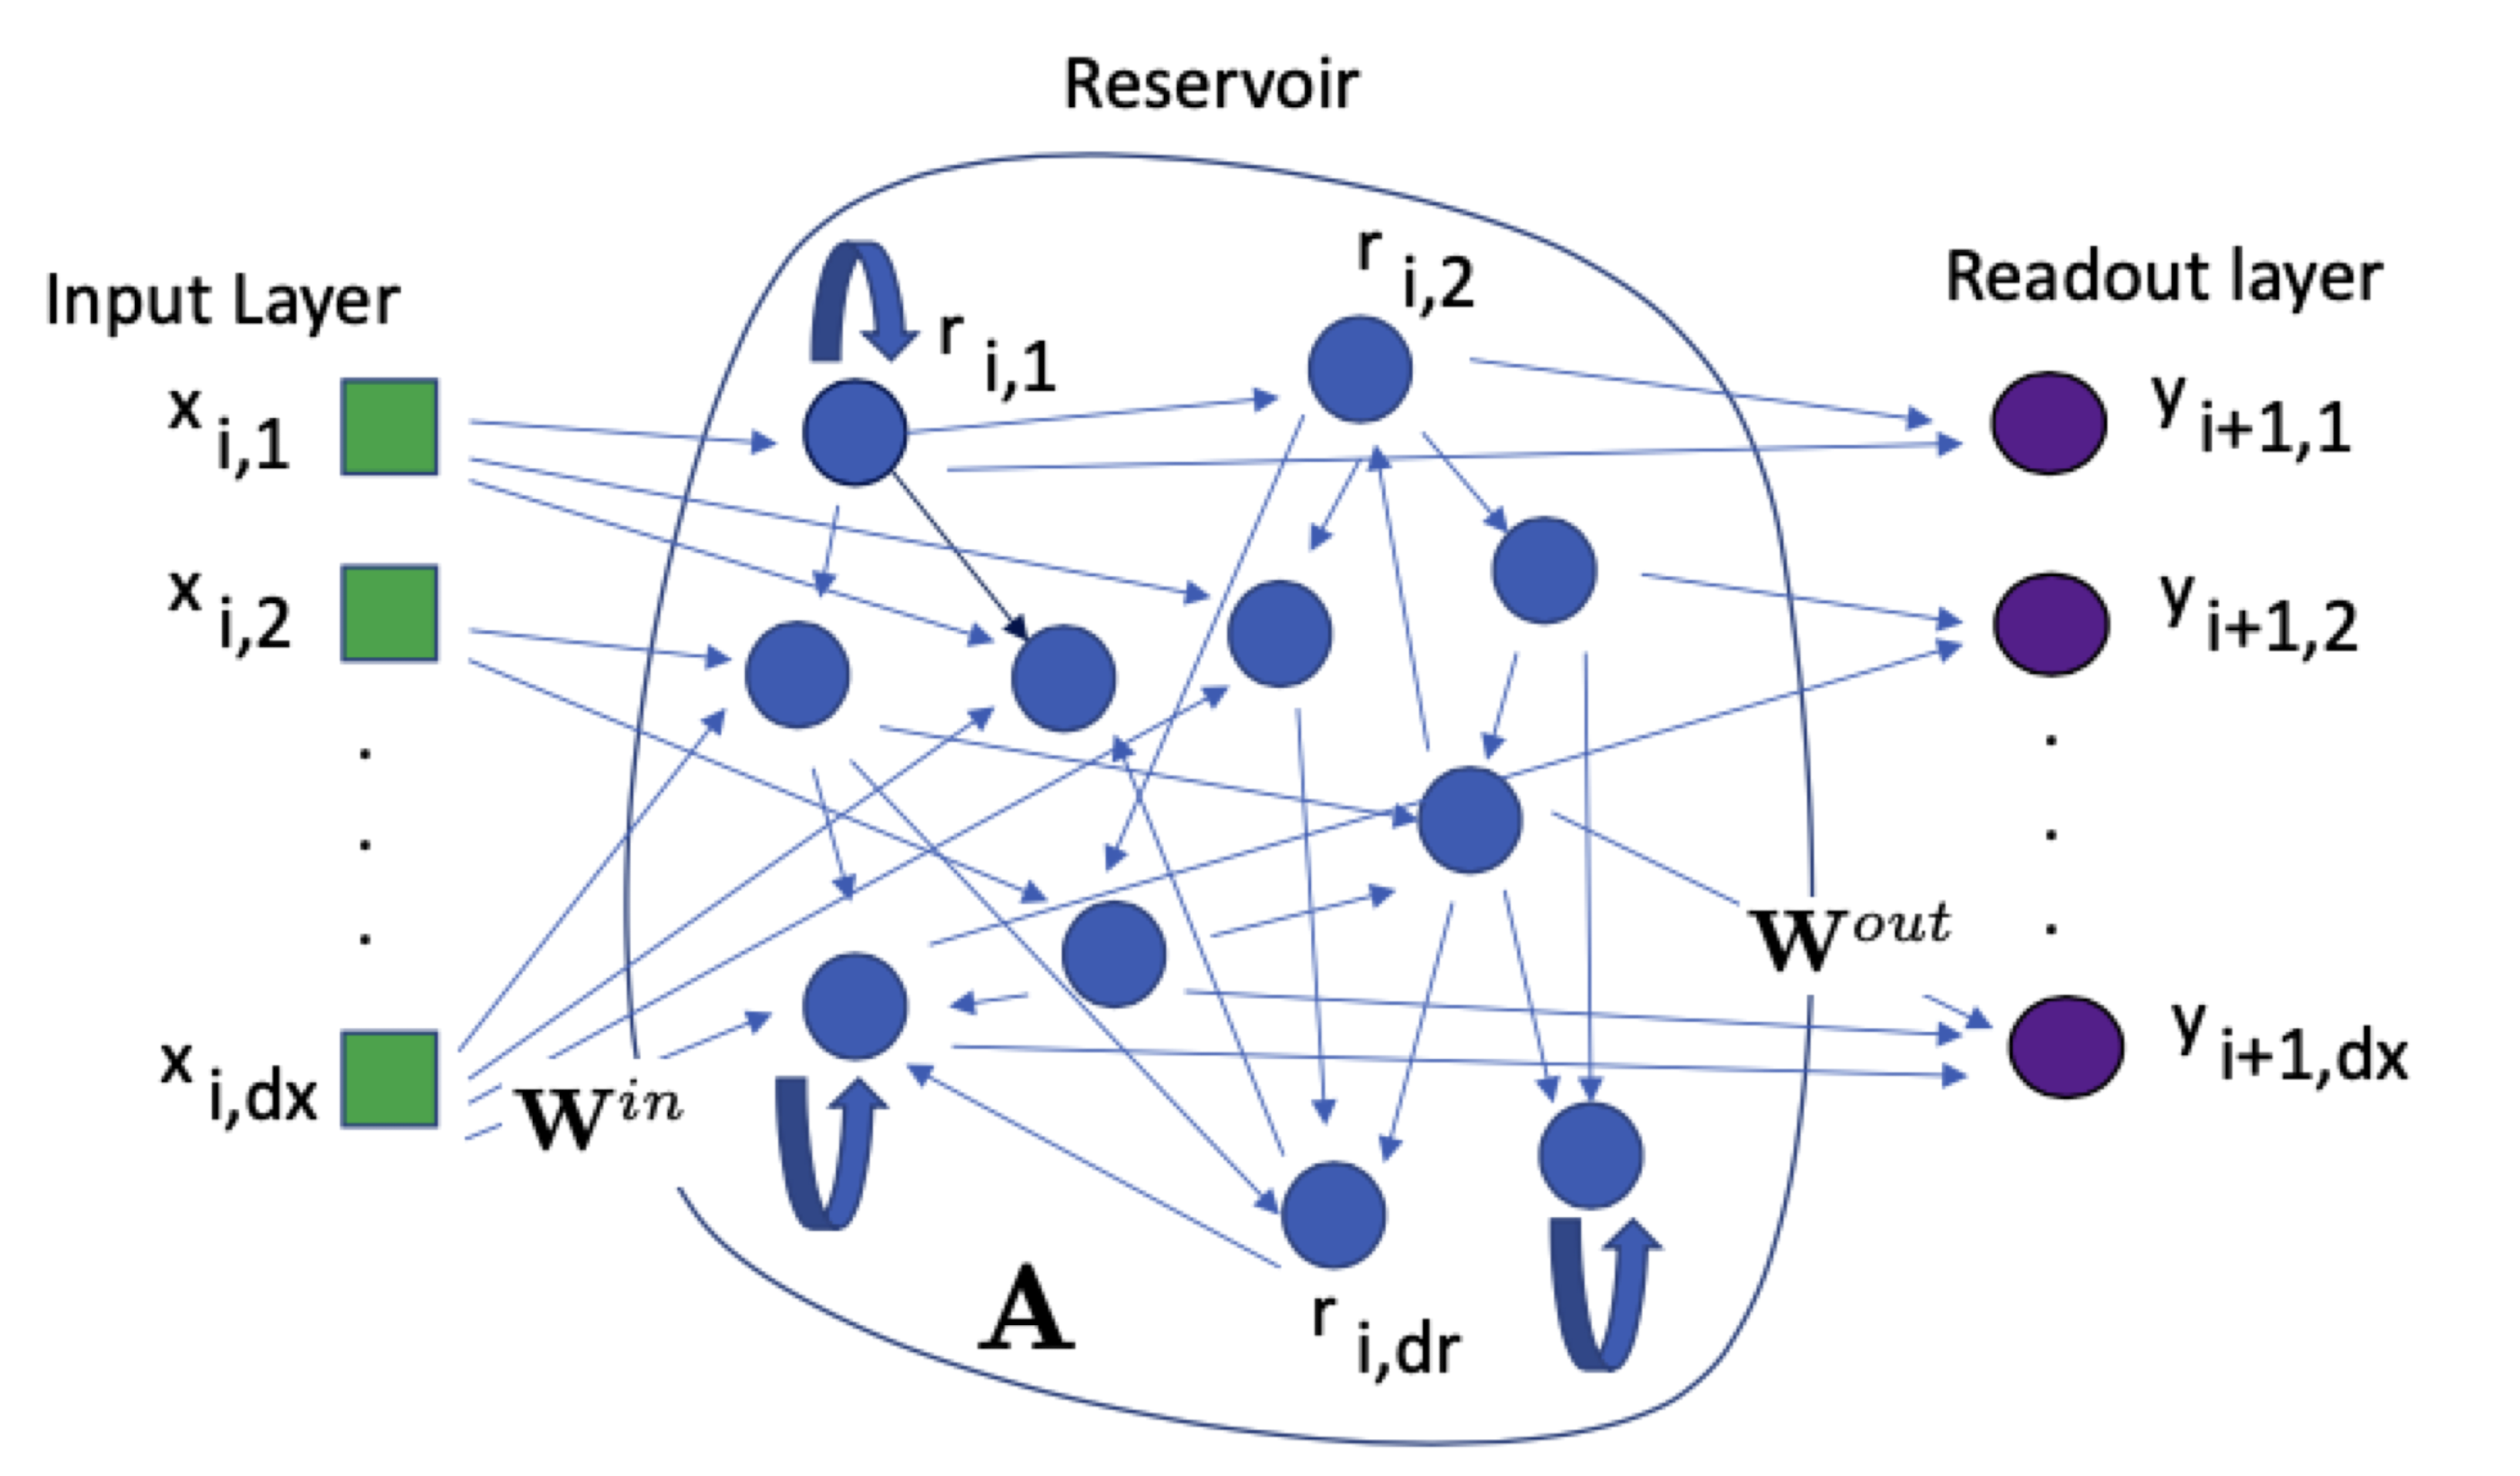
\includegraphics[width=\textwidth]{Fig/bollt_reservoir.png}
                \caption{\scriptsize{Reservoir Computer の各層の関係} \\ \tiny{Fig. 2 from \cite{Bollt}}}
            \end{figure}
        \end{column}
      \end{columns}
\end{frame}



\subsection{Reservoir Computer に関する理論}
\begin{frame}
    
\end{frame}

\subsection{先行研究}
\begin{frame}
    
\end{frame}

\subsection{Hyperparameters の最適化}
\begin{frame}{Reservoir に関する Hyperparameters}
    Reservoir に関する Hyperparameter のうち,最適化の対象としたものを記した.説明は,\cite{rpy_doc}の Tutorial 4 を参考にした.
    \begin{enumerate}
        \item Cell Number (N): セル数.
        \item spectral radius (sr): スペクトル半径.Reservoir の 行列 $\mathcal{W}$ の固有値の絶対値の最大値.\begin{itemize}
            \item 小さいと安定したダイナミクス、大きいとカオス的なダイナミクス.
            \item 理論的には$1$ に近いと Reservoir の初期条件に影響を受けにくく,良好な memory を持つことが推測される.
        \end{itemize}
        \item input scaling (iss): Reservoir の入力 $\mathcal{W}_{in}$ に適用される係数.入力にゲインを加える.\begin{itemize}
            \item 高くするとReservoir と 入力の相関を(飽和点まで)高める.
            \item 低くすると Reservoir は外部の入力より自身のダイナミクスに強く影響を受ける.
            \item 多変量時系列データの各変数の影響度を調整可能.
        \end{itemize}
        \item leaking rate (lr): 次ステップの決定に際しての現在の状態と新しい入力の影響度の割合.\begin{itemize}
            \item 高い(低い)と惰性が高く(低く),過去の記憶状態が高く(低く)なる.
            \item ESN のネットワークがその状態を変化させる速度を制御する.
        \end{itemize}
        \item ridge (ridge): 
    \end{enumerate}
\end{frame}

\begin{frame}{Hyperparameters 最適化のアルゴリズム}
    Hyperparameters の最適化には python ライブラリである Optuna を用いた.
     
    Optunaで実装されている Hyperparameters の最適化アルゴリズムは例えば以下がある.
    \begin{columns}[T] % [T] は列を上部で揃えるオプション
        \begin{column}{.5\textwidth}
            

            \begin{block}{optuna.samplers: from \cite{optuna_doc}}
                \begin{enumerate}
                    \item \textbf{optuna.samplers.RandomSampler}: ランダムサンプリングを使用するサンプラー。
                    \item \textbf{optuna.samplers.TPESampler}: TPE(Tree-structured Parzen Estimator)アルゴリズムを使用するサンプラー。
                    \item \textbf{optuna.samplers.CmaEsSampler}: CMA-ES(Covariance Matrix Adaptation Evolution Strategy)をバックエンドとして使用するサンプラー。
                \end{enumerate}
                
            \end{block}
        
        \end{column}
        \begin{column}{.5\textwidth}
            \begin{itemize}
                \item この研究では,CmaEsSampler (最終的に採用), TPESampler と hyperopt という別のpython ライブラリの random search を用いた.\begin{itemize}
                    \item 経験的に,その順により好ましい best value を与えた.
                    
                \end{itemize}
                \item また,Optuna搭載の pruner も利用した.\begin{itemize}
                    \item 見込みの悪い Hyperparameters のセットを見限ること.
                    \item 使用したのは SuccessiveHalvingPruner.
                \end{itemize}
                \item なお,hyperopt には Optunaのいくつかの機能は搭載されていない.
            \end{itemize}
        \end{column}
      \end{columns}


\end{frame}


\subsection{実験のパラメータ設定}

\begin{frame}
    \begin{columns}[T] % [T] は列を上部で揃えるオプション
        \begin{column}{.5\textwidth}
            \begin{itemize}
                \item Rössler系の数値シミュレーション\begin{itemize}
                    \item $A = 1.0$ 
                    \item $a = 0.2,\ b = 0.2,\ c = 5.7.$ 
                    \item 初期条件:$\left[ X_0, Y_0, Z_0 \right] = [1.0, 1.0, 1.0]$ 
                    \item 時間範囲:$t_\text{span} = [0, 4510].$ 
                    \item 位相シフト時間:$p = 8$ に対して Hyperparameter を最適化. 
                    \item 注.配列データは $1$ タイムステップに対して $10$ 個データポイントをとって生成したので,長さ $[0, 45100]$ である.
                \end{itemize}
                \item Optunaの最適化
                \begin{itemize}
                    \item $\text{nb seeds} = 3$
                    \item $\text{nb trials} = 3000$ 
                    \item 最適化アルゴリズム:CmaEsSampler
                    \item pruner: SuccessiveHalvingPruner
                    \item $\text{train len} = 20000$
                    \item $\text{test len} = 10000$
                \end{itemize}
            \end{itemize}
        \end{column}
        \begin{column}{.5\textwidth}
            \begin{itemize}
                \item Hyperparameters の探索空間\begin{itemize}
                    \item N = 10000: 固定

                    sr:  (1e-2, 10, log = True)

                    lr: (1e-3, 1, log = True)

                    iss: (0, 1)
                    
                    ridge: (1e-9, 1e-2, log = True)

                    \item 一様ランダムにサンプリング.
                    \item log = True で$\log$ をとって一様ランダムにサンプリング.
                \end{itemize}
                \item 採用した Hyperparameters のセット\begin{itemize}
                    \item Best value: 0.0017332259260817507
                    Best parameters: {
                        
                        'sr': 0.568437354122632, 
                        
                        'lr': 0.33989147591891816, 
                        
                        'iss': 0.08827385538440446, 
                        
                        'ridge': 1.30084237042553e-08}
                \end{itemize}
            \end{itemize}
        \end{column}
      \end{columns}
    
\end{frame}


\begin{frame}{参考文献 - 1}
    \begin{thebibliography}{99}    
        \bibitem[1]{Bollt}
        Bollt, E.M. (2020). On explaining the surprising success of reservoir computing forecaster of chaos? The universal machine learning dynamical system with contrast to VAR and DMD. Chaos, 31 1, 013108 .

        \bibitem[2]{Trouvain}
        Trouvain, N., Pedrelli, L., Dinh, T. T., Hinaut, X. (2020) Reservoirpy: an efficient and user-friendly library to design echo state networks. In International Conference on Artificial Neural Networks (pp. 494-505). Springer, Cham.

        \bibitem[3]{Yamaguchi et al.}
        Yamaguchi, Y., Suzuki, T., Mizoro, Y., Kori, H., Okada, K., Chen, Y., Fustin, J. M., Yamazaki, F., Mizuguchi, N., Zhang, J., Dong, X., Tsujimoto, G., Okuno, Y., Doi, M., and Okamura, H. (2013). Mice genetically deficient in vasopressin V1a and V1b receptors are resistant to jet lag. Science (New York, N.Y.), 342(6154), 85–90. 
    \end{thebibliography}
\end{frame}

\begin{frame}{参考文献 - 2}
    \begin{thebibliography}{99}    
        \bibitem[4]{optuna_doc}
        Optuna. (2018). Optuna Documentation. Retrieved from \url{https://optuna.readthedocs.io/en/stable/} [Accessed on: \today]

        \bibitem[5]{rpy_doc}
        ReservoirPy Team. (Year). ReservoirPy Documentation. Retrieved from \url{https://reservoirpy.readthedocs.io/en/latest/} [Accessed on: \today].

    \end{thebibliography}
\end{frame}
